\Exhibit{ComposerWikipedia}{%
    Статья в Wikipedia о `Composer (Software)', подтверждающая адрес репозитория `Packagist'%
}

Это скриншот статьи в Wikipedia о `Composer (Software)'.
Его цель -- объяснить, что такое `Packagist'
(потому у что Packagist нет отдельной страницы в Wikipedia).

Здесь сказано:

\Quote{%
    Composer запускается из командной строки и устанавливает зависимости (библиотеки) приложения.
    Он также позволяет устанавливать приложения PHP, доступные в `Packagist'[5] --
    главном репозитории пакетов.%
}

Это доказывает, что Packagist -- главный источник пакетов PHP,
и поэтому он является источником статистик их загрузки.

Внизу страницы ссылка (номер 5) ведёт на packagist.org --
источник статистики в \ExhibitRef{PhpStanPackagist}.

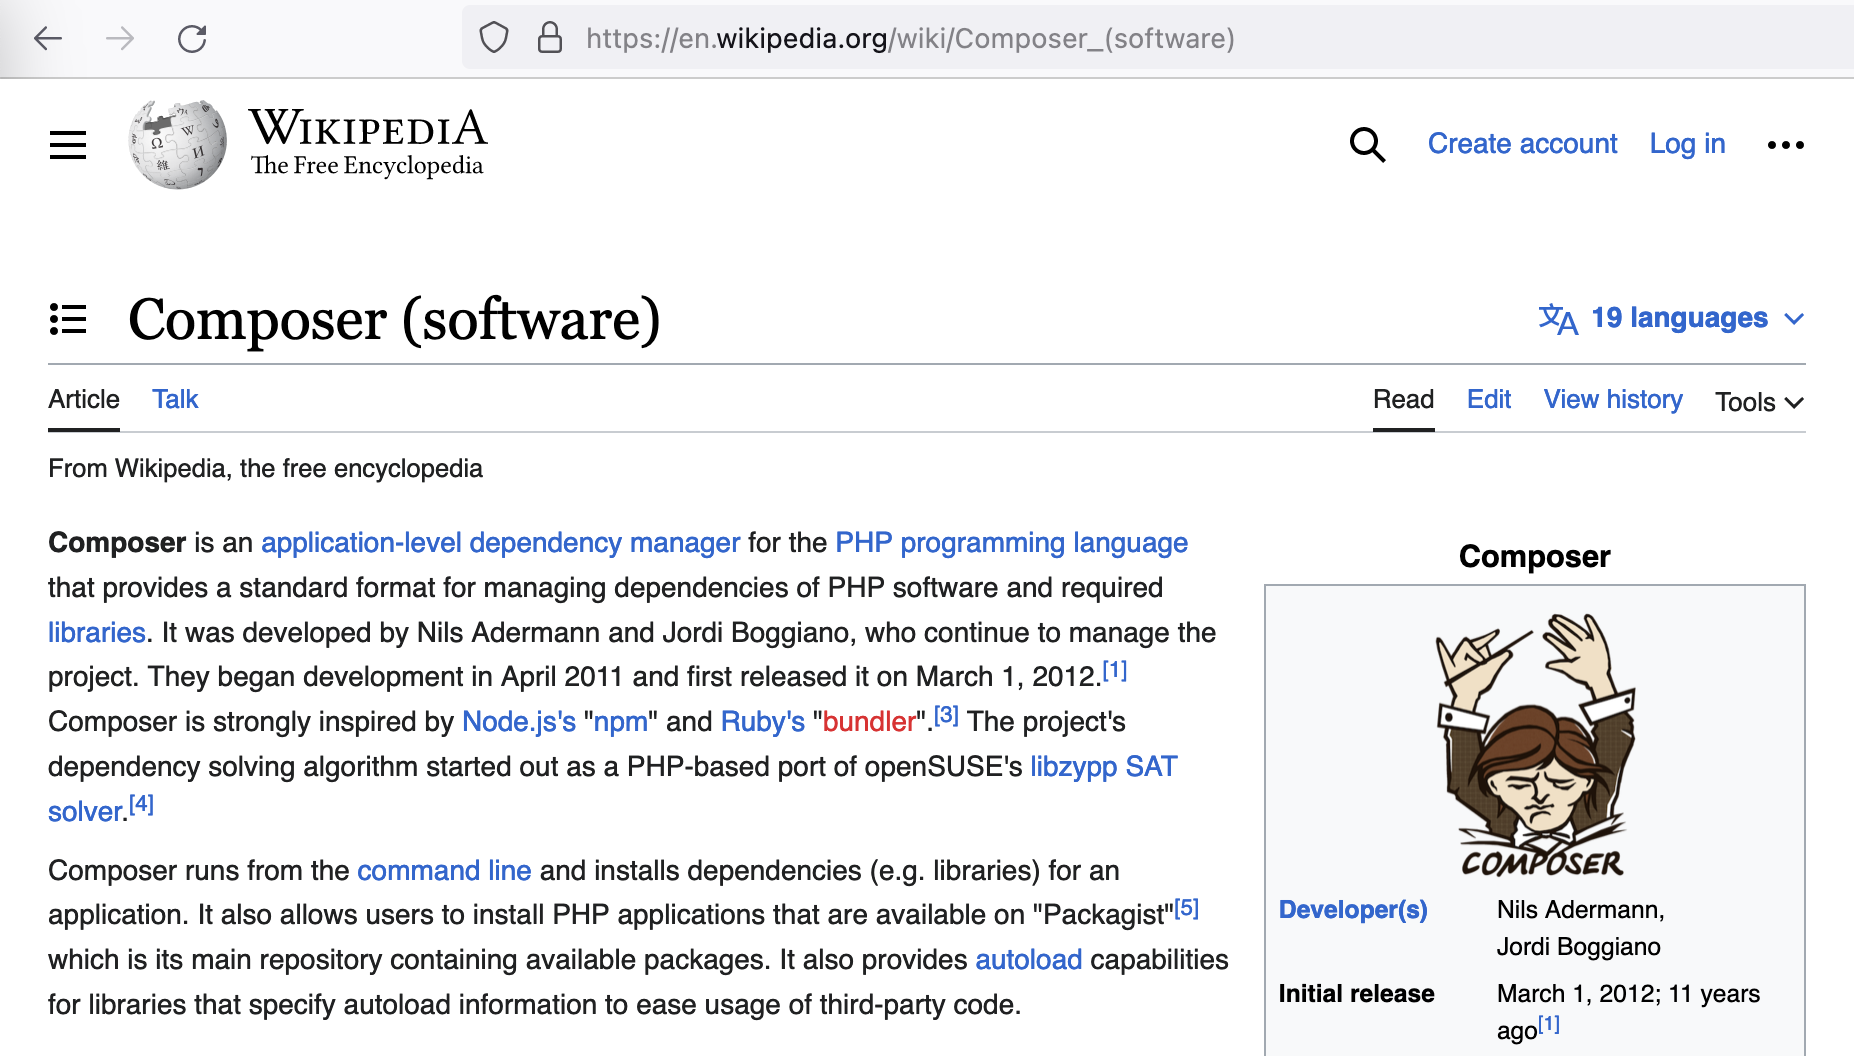
\includegraphics[width=\textwidth]{packagist-wikipedia-p1}
\CenterParentheses{Середина пропущена}

\pagebreak

\CenterParentheses{Середина пропущена}
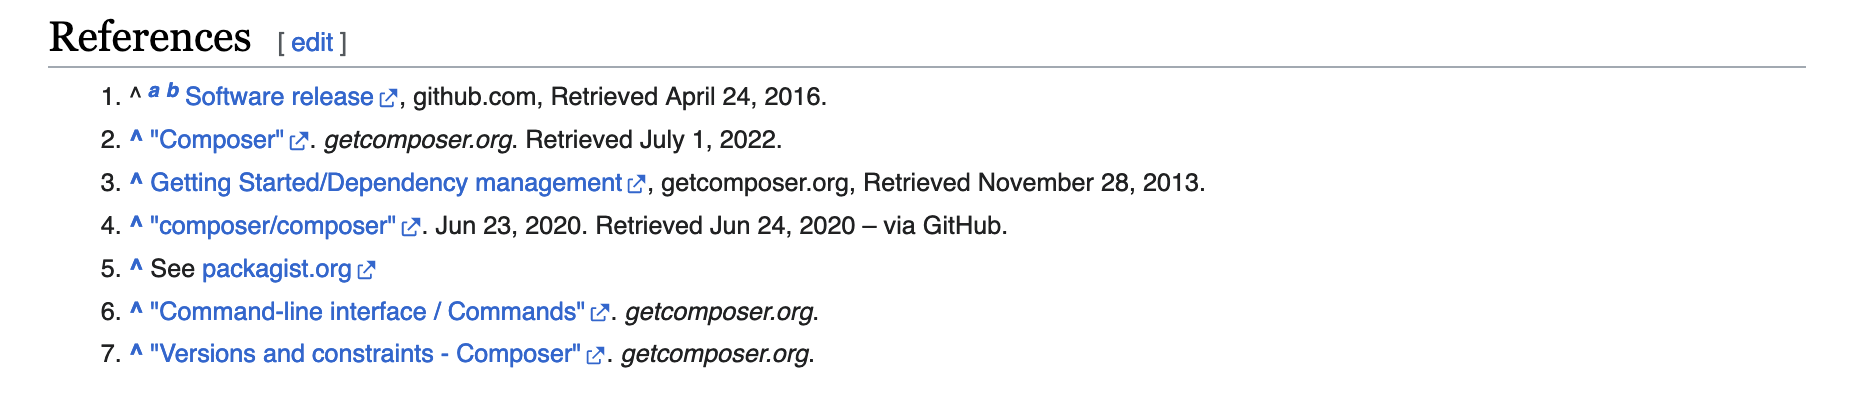
\includegraphics[width=\textwidth]{packagist-wikipedia-bottom}

\pagebreak




